\documentclass{article}
\usepackage[utf8]{inputenc}
\usepackage[backend=biber]{biblatex}
\usepackage{amssymb}
\usepackage{amsmath}
\usepackage{dsfont}
\addbibresource{bib.bib}
\setlength{\parindent}{0em}
\bibliography{bib}
\setlength{\parskip}{6pt}
\usepackage[margin=1.0in]{geometry}
\usepackage{graphicx}
\usepackage{caption}
\usepackage{subcaption}
\usepackage{wrapfig}
\usepackage{url}

\title{Intro to deep learning with PyTorch}
\author{Miguel A. Saavedra-Ruiz}
\date{May 2020}
\linespread{1.0}

\nocite{*}


\begin{document}

\maketitle

\section*{Autoencoders}

The autoencoder is a very simple neural network and it is similar to the multi-layer perceptron. This network architecture is designed to reproduce its input at the output layer. The main differences between an Autoencoder and a MLP is that the number of input neurons is equal to the number of output neurons. 

\begin{figure}[ht]
    \centering
    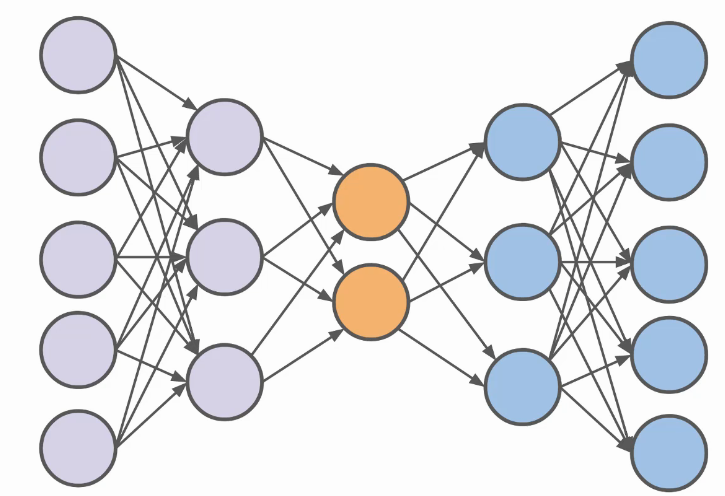
\includegraphics[width=0.35\textwidth,height=0.35\textheight,keepaspectratio]{images/auto.png}
    \captionsetup{justification=centering}
    \caption{Autoencoder with three hidden layers}
    \label{fig:f1}
\end{figure}

Fig. \ref{fig:f1} presents a simple stacked autoencoder with three hidden layers. As it is possible to see that the output size is the same as the input size. One important thing to note in that in the left size of the image the model starts with five input neurons and then then that gets reduced to three neurons in the first hidden layer and then to two in the second hidden layer. Subsequently, it gets gradually increased until the output layer has the same number of neurons as the input layer.

\begin{figure}[ht]
    \centering
    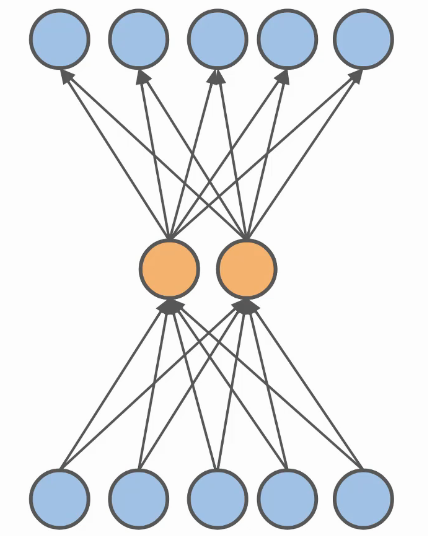
\includegraphics[width=0.25\textwidth,height=0.25\textheight,keepaspectratio]{images/simple_auto.png}
    \captionsetup{justification=centering}
    \caption{Autoencoder with one hidden layer}
    \label{fig:f2}
\end{figure}

To explain the basic idea behind an autoencoder let's use a simpler model presented in Fig. \ref{fig:f2}. This model basically has one hidden layer and then the output has the same dimension as the input layer. For the sake of notation, see Fig. \ref{fig:f3} which is another representation of the same model presented in Fig. \ref{fig:f2}. Recall that an autoencoder is a feedforward network that is trained to reproduce its input at the output. Therefore, what this network architecture is trying to do is directly mimic its input at the output layer.


As it is possible to notice, \(W\) are the weights between the input layer and the hidden layer, \(b\) is the bias term of the hidden layer and \(h(x)\) is the output of the hidden layer. Furthermore, \(W^{out}\) are the weights between the output layer and the hidden layer, \(c\) is the bias term of the output layer and \(\overline{x}\) is the output of the final layer Fig. \ref{fig:f3}. 

\begin{figure}[ht]
    \centering
    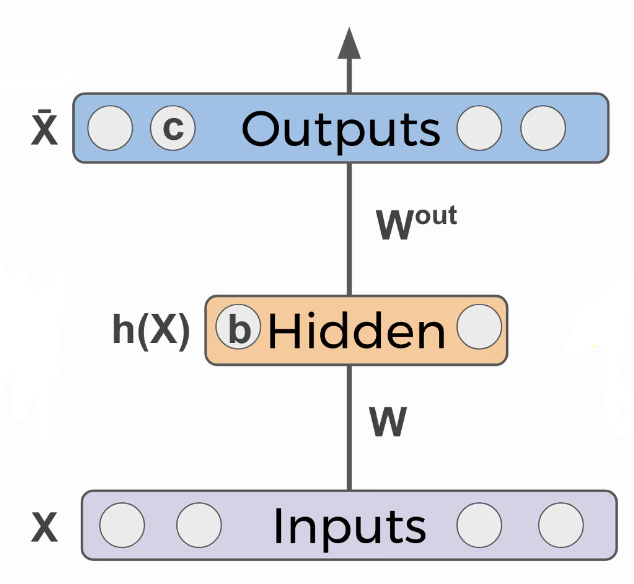
\includegraphics[width=0.35\textwidth,height=0.35\textheight,keepaspectratio]{images/architecture.png}
    \captionsetup{justification=centering}
    \caption{Representation of autoencoder with one hidden layer}
    \label{fig:f3}
\end{figure}

Mathematically, the equations for an autoencoer are exactly the same as the ones for an MLP. In this case, for the hidden layer the equation is given by \eqref{eq:2} and for the output layer is \eqref{eq:2}. There are two main parts in an Autoencoder and that is the first chunk of the autoencoder that goes from the input layer to the hidden layer (Encoder) and the second part which goes from the hidden layer to the output layer (Decoder). Hence, the encoder equation for the autoencoder presented in Fig. \ref{fig:f2} is given by \eqref{eq:1} and for the decoder by \eqref{eq:2}.

\begin{equation}
h(x) = \sigma(Wx + b)
\label{eq:1}
\end{equation}

\begin{equation}
\overline{x} = \sigma(W^{out}h(x) + c)
\label{eq:2}
\end{equation}

The main function of the encoder section is to find a compressed representation of the input layer. On the other hand, the function of the decoder is reproduce the input layer at the output. A really common practice with autoencoders is to use tied weights. This means that the weights coming from the input to the hidden layer are going to be the same weights between the hidden and output layer but transposed \(W^{out} = W^T\). This approach is possible owing to the autoencoder is basically train to reproduce the input at the output layer. It is important to mention that the only thing tied are the weights, the bias are not tied.

The key idea in an autoencoder is that the encoder section is trying to create an internal representation that maintains all the information of the input. The really important aspect about the encoder layer is that it is possible to use it to extract meaningful features from the input data and create a compressed representation. Owing to this benefit of the encoder, Autoencoders have been used for principal components analysis (PCA).

An Stacked autoencoder is the one presented in Fig. \ref{fig:f1} and it basically has more hidden layers and a bigger ability for abstraction.

One of the biggest advantages of autoencoders is that they learn a pretty descent representation of the weights of the a network just with the input. The autoencoders can be used as a initializer and then use the learned weights as the initial ones for a fine-tuning process. This kind of approach have shown good results and ease the training procedure of neural networks.


\printbibliography


\end{document}
